\section{Reference implementation}
\label{sec:implementation}

In this section we briefly describe a reference implementation of the
models introduced in Sections~\ref{sec:model:TSMS}
and~\ref{sec:MTSMS}. This implementation is given as a proof of
concept and do not seeks to be an efficient nor a complete database
system. We implemented the \acro{TSMS} and \acro{MTSMS} models using
then Python~\cite{python:doc2} programming language.

The implementations of the two models, \acro{TSMS} and \acro{MTSMS},
are organized respectively in two separated Python libraries:
\texttt{Pytsms} and \texttt{RoundRobinson}.  \texttt{RoundRobinson}
has a strong dependency on \texttt{Pytsms} following the dependency of
\acro{MTSMS} on \acro{TSMS}.  The code of this implementation can be
found at~\cite{llusa:roundrobinson}.

The reference implementation follows the object orientated paradigm
and it observes a clear mapping between the model and the object
classes. Unified Modeling Language~(\acro{UML}) diagrams are used to
define the classes structure.  Operations are implemented as object
methods, which are not show in \acro{UML} diagrams for space reasons.


\subsection{Pytsms}

\texttt{Pytsms} is the reference implementation for the model concepts
of measure, time series and temporal representation function.
Figure~\ref{fig:implementacio:pytsms-uml} shows the relationships
among these objects in a \acro{UML} diagram. A \texttt{TimeSeries}
object is an aggregation of \texttt{Measure}
objects. \texttt{TimeSeries} and \texttt{Representation} objects have
a relation of association, that is each \texttt{TimeSeries} has a
default representation and a \texttt{Representation} operates over a
\texttt{TimeSeries}.

%\tikzsetnextfilename{fig_pytsms_uml}
\begin{figure}[tp]
  \centering
  %  \begin{tikzpicture}

  %Timeseries
  \umlsimpleclass[x=0,y=0] {TimeSeries}{}{}

  % Measure
  \umlclass[x=-1.5,y=-2] {Measure}{}{}
  \umluniaggreg[mult=0..*]  {TimeSeries}{Measure}
  %\umlclass[x=-5.2,y=-2] {MFloat}{}{}
  %\umlclass[x=-2.8,y=-2] {MChar}{}{}
  %\umlinherit {MFloat}{Measure}
  %\umlinherit {MChar}{Measure}

  %Repr
  \umlclass[x=3.5] {Representation}{}{} %,type=abstract
  \umlassoc[mult1=1,mult2=1]  {TimeSeries}{Representation}
  \umlclass[x=2.5,y=-2] {Zohe}{}{}
  \umlclass[x=4.5,y=-2] {Dd}{}{}
  \umlinherit {Zohe}{Representation}
  \umlinherit {Dd}{Representation}

  %Associacions
  \umlclass[x=-1.25,y=-4] {RegularProp}{}{}
  \umluniassoc  {TimeSeries}{RegularProp}
  \umlclass[x=1.25,y=-4] {Storage}{}{}
  \umluniassoc {TimeSeries}{Storage}

  %Dependencies
  \umlemptypackage[x=4,y=-5]{Matplotlib}
  \umldep{Zohe}{Matplotlib}
  \umldep{Dd}{Matplotlib}


  \end{tikzpicture}

  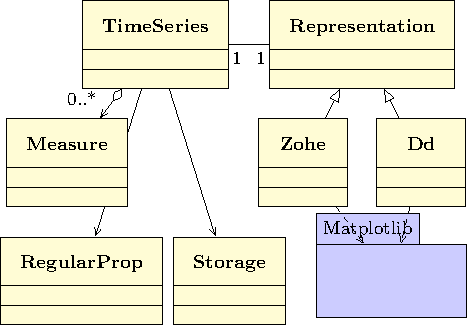
\includegraphics{fig_pytsms_uml.pdf}
  \caption{Pytsms \acro{UML} class diagram}
  \label{fig:implementacio:pytsms-uml}
\end{figure}


A \texttt{TimeSeries} object has a big amount of methods. We classify
them based on their functionality. First, a \texttt{TimeSeries} object
includes methods to manipulate the structural model. We implement
\texttt{TimeSeries} as a subclass of the predefined \texttt{set}
Python type. Second, a \texttt{TimeSeries} object has methods that
implement set, sequence and temporal function operators as described
in Section~\ref{sec:model:operations}.  Third, accessory operations of
\texttt{TimeSeries} are grouped into two visitor objects:
\texttt{RegularProp} groups the regularity operation definitions and
\texttt{Storage} has methods for storing and retrieving time series
from the file system. Recall that visitor is a pattern design that
allows new functionality to be added to objects without modifying the
objects~\cite{ziade08:expert_python_programming:visitor,martin02:visitor}.

Figure~\ref{fig:implementacio:pytsms-uml} shows two specialisations
for \texttt{Representation} that refer to the representation functions
given in Section~\ref{sec:model:tfunc}. Basically, each actual
\texttt{Representation} defines the graph and the temporal interval
operation. Furthermore, there is also a method to plot coherently the
time series to its representation; for which we use the Python
\emph{Matplotlib} library.
%
% Aqui hi els temes que he comentat en la revisio de la primera part
% SBS



\begin{example}
  \label{ex:pytsms:example}
  In this example we reproduce an interpreter session working with
  \texttt{Pytsms}. First we define the two time series \texttt{s1} and
  \texttt{s2} from Example~\ref{ex:model:s1s2} and after that we apply
  different operations: union, temporal union, concatenation, closed
  interval, \zohe{} temporal interval, \zohe{} temporal selection, and
  the test of regular property. Note that \texttt{Measure} is
  abbreviated to \texttt{m}. The log of the session is as follows:

  {\small
\begin{verbatim}
# Import the required objects
>>> from pytsms import TimeSeries, Measure as m
>>> from pytsms.representation import Zohe
>>> from pytsms.properties import isRegular

# Define the two time series
>>> s1 = TimeSeries([m(1,1),m(3,1),m(4,0),m(5,1)])
>>> s2 = TimeSeries([m(2,2),m(3,2),m(4,0),m(6,2)])

# Manipulate the two time series
>>> s1.union(s2)
TimeSeries([m(1,1), m(2,2), m(3,1), 
            m(4,0), m(5,1), m(6,2)])
>>> s1.union_temporal(s2)
TimeSeries([m(1,1), m(2,2), m(4,0), m(5,1), m(6,2)])
>>> s1.concatenate(s2) 
TimeSeries([m(1,1), m(3,1), m(4,0), m(5,1), m(6,2)])
>>> s2.interval_closed(2,5)
TimeSeries([m(2,2), m(3,2), m(4,0)])
>>> s2.interval_temporal(2,5,Zohe)
TimeSeries([m(3,2), m(4,0), m(5,2)])

# Check for regularity
>>> s2.accept(isRegular())
False
# regularise to {0,2,4} by Zohe method
>>> r2 = s2.selection_temporal(range(0,6,2),Zohe)
>>> r2
TimeSeries([m(0,2), m(2,2), m(4,0)])
>>> r2.accept(isRegular())
True
\end{verbatim}
}
\end{example}





\subsection{RoundRobinson}

\texttt{RoundRobinson} is the reference implementation for the
multiresolution time series model. It includes objects like
resolution subseries, buffers, discs, and attribute aggregate
functions. Figure~\ref{fig:implementacio:roundrobinson-uml} shows the
relationships among these objects in a \acro{UML} diagram. 
%
A \texttt{MultiresolutionSeries} object is an aggregation of
\texttt{Resolution} objects. A \texttt{Resolution} is composed by one
\texttt{Buffer} and one \texttt{Disc}. Each \texttt{Buffer} is
associated to one \texttt{TimeSeries}, from the \texttt{Pytsms}
library, and each \texttt{Disc} is associated to another
\texttt{TimeSeries}, which respectively are the buffer's
and the disc's time series in the \acro{MTSMS} model. Furthermore, each
\texttt{Buffer} is associated to one attribute aggregate function
which is defined as a \texttt{Python} function with two parameters: a
\texttt{TimeSeries} \texttt{s} and a consolidation time interval
\texttt{i}.

%\tikzsetnextfilename{fig_roundrobinson_uml}
\begin{figure}[tp]
  \centering
  %\begin{tikzpicture}

  %MultiTimeseries
  \umlsimpleclass[x=0,y=0] {MultiresolutionSeries}{}{}  
  %\umlclass[x=-4,y=0] {Set}{}{}
  %\umlinherit{MultiresolutionSeries}{Set}
  %Components 
  \umlclass[x=0,y=-2] {Resolution}{}{}
  \umluniaggreg  {MultiresolutionSeries}{Resolution}
  %SubComponents 
  \umlclass[x=-1.2,y=-4] {Buffer}{}{}
  \umlclass[x=1.2,y=-4] {Disc}{}{}
  \begin{umlpackage}[x=-3,y=-6.6]{aggregators}
    \umlclass[template={s,i}] {Function}{}{}
  \end{umlpackage}
  \umlunicompo[mult=1]  {Resolution}{Buffer}
  \umlunicompo[mult=1]  {Resolution}{Disc}
  \umluniassoc[mult=1]  {Buffer}{Function}

  %TimeSeries
  \begin{umlpackage}[x=1,y=-6.5]{Pytsms}
    \umlclass{TimeSeries}{}{}  
  \end{umlpackage}
  \umluniassoc[mult=1]  {Buffer}{TimeSeries}
  \umluniassoc[mult=1]  {Disc}{TimeSeries}

  %Associacions
  \umlclass[x=-3.25,y=-2.7] {Storage}{}{}
  \umluniassoc {MultiresolutionSeries}{Storage}
  \umlclass[x=-3.5,y=-1] {Plot}{}{}
  \umluniassoc {MultiresolutionSeries}{Plot}

\end{tikzpicture}

  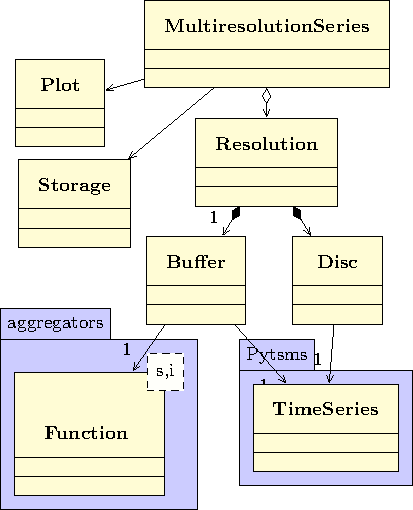
\includegraphics{fig_roundrobinson_uml.pdf}
  \caption{RoundRobinson \acro{UML} class diagram}
  \label{fig:implementacio:roundrobinson-uml}
\end{figure}


\texttt{MultiresolutionSeries} is a subclass of the predefined
\emph{Set} Python class. It adds complementary operations that are
grouped into two objects: \texttt{Storage}, that has methods to store
and retrieve multiresolution time series from the file system and
\texttt{Plot}, that has methods to plot the time subseries of the
multiresolution schema.


\texttt{MultiresolutionSeries} has a method \texttt{addResolution} to
define the multiresolution schema structure by adding resolution
subseries. Every new resolution is configured by four parameters:
\texttt{delta}, \texttt{k}, \texttt{f}, and \texttt{tau} that allow to
create the corresponding buffer and disc.
\texttt{MultiresolutionSeries} has methods \texttt{add},
\texttt{consolidable}, and \texttt{consolidate} that operate on the
corresponding methods of the contained resolution subseries.


\texttt{MultiresolutionSeries} can be queried using one of two
methods: \texttt{seriedisc} and \texttt{totalseries}. The method
\texttt{seriedisc} returns the \texttt{TimeSeries} corresponding to
the disc identified by the parameters \texttt{delta} and
\texttt{f}. The method \texttt{totalseries} returns the \texttt{TimeSeries} that
results from the concatenation of all \texttt{seriedisc} sorted by
\texttt{delta}.
% as there can not be repeated \emph{delta}, \emph{totalseries} has a
% parameter \emph{f} for selecting only \emph{discSeries} with a
% determined attribute aggregate function.

In the module \texttt{aggregators} we have implemented some default
attribute aggregate functions. Moreover, users can define new
aggregators as well. For instance, we defined the \zohe{} aggregate
functions explained in Section~\ref{sec:model:interpolador}, which
basically aggregate over the temporal interval
\verb|s.interval_temporal(s,t,Zohe)|. This is shown in
Example~\ref{ex:pytsms:example}.


\begin{example}
  In this example we define using \texttt{Pytsms} the time series
  \texttt{S}. Also, using \texttt{RoundRobinson} we define the
  multiresolution time series $M$ from
  Example~\ref{ex:model:smultiresolution}. Then, we apply
  consolidation and we query the result.

{\small
\begin{verbatim}
# Import the required objects
>>> from pytsms import TimeSeries, Measure as m
>>> from roundrobinson import MultiresolutionSeries
>>> from roundrobinson.aggregators import mean_zohe,
...                                       maximum_zohe

# Define the original time series
>>> s = TimeSeries([m(1,6),m(5,2),m(8,5),m(10,0),
...                 m(14,1),m(19,6),m(22,11),
...                 m(26,6),m(29,0)])

# Define the multiresolution time series
>>> M = MultiresolutionSeries()
# Define the multiresolution schema
>>> M.addResolution(delta=5,k=4,f=mean_zohe,tau=0)
>>> M.addResolution(delta=10,k=2,f=maximum_zohe,tau=0)

# Add the measures
>>> for m in s: M.add(m)
# M is consolidable
>>> M.consolidable()
True
# Consolide until no more consolidable
>>> while M.consolidable():
...    M.consolidate()

# Query the consolidated discs 
>>> M.seriedisc(5,mean_zohe)
TimeSeries([m(10,3), m(15,2), m(20,7), m(25,8)])
>>> M.seriedisc(10,maximum_zohe)
TimeSeries([m(10,6), m(20,11)])
# Query the total time series
>>> M.totalseries()
TimeSeries([m(10,3), m(15,2), m(20,7), m(25,8)])
\end{verbatim}
}
\end{example}





%%% Local Variables:
%%% TeX-master: "main"
%%% ispell-local-dictionary: "british"
%%% End:
